\section{Error Analysis}
\label{sec:error}

% All analyses use TEST predictions of the final model (E7 seed 1) and of the CE
% winner (E3); no decision in this section feeds back into model selection.

\subsection{Confusion Structure}

The row-normalized test confusion matrix of the final model
(Fig.~\ref{fig:confusion}) has five dominant off-diagonal patterns.
(i)~\emph{Water} is recalled only 6\% of the time: 54\% of its pixels are
predicted as \emph{mulch} and 22\% as \emph{grass}. (ii)~\emph{Rock-bed} goes
to mulch (41\%) or gravel (39\%). (iii)~\emph{Bush} splits between grass (36\%)
and tree (32\%). (iv)~Small obstacles are absorbed by their surroundings:
\emph{sign} (57\%) and \emph{pole} (29\%) are predicted as tree, \emph{person}
as tree, vehicle, or picnic-table. (v)~\emph{Dirt} goes to mulch (33\%) and
grass (21\%). Overall, 61\% of misclassified test pixels cross a traversability
group, and the most consequential crossing is safety-relevant: in the group
confusion, 55\% of water pixels are labeled \emph{smooth ground} and 34\% of
rough ground is also labeled smooth ground. A planner trusting these labels
would treat the creek as an easy trail.

\begin{figure}[t]
  \centering
  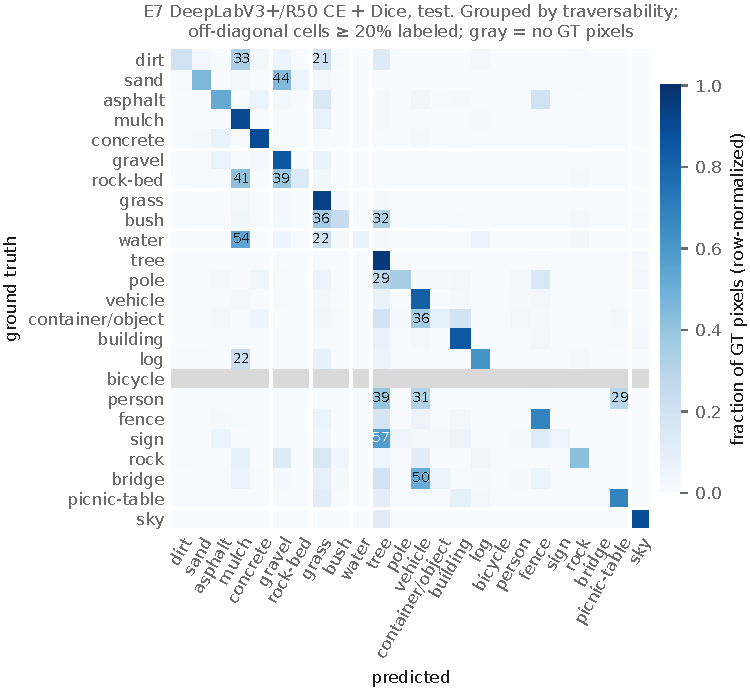
\includegraphics[width=\linewidth]{../results/figures/confusion_e7_ce_dice_s1_test.pdf}
  \caption{Row-normalized confusion matrix of the final model on RUGD test,
  classes ordered by traversability group. Water and rock-bed collapse into
  mulch and gravel; bush splits between grass and tree; thin objects are
  absorbed by \emph{tree}.}
  \label{fig:confusion}
\end{figure}

\subsection{Hardest Frames and Sequences}

Per-sequence test mIoU of the final model is 44.4\% on \emph{park-1}, 36.2\%
on \emph{trail-13}, 29.8\% on the motion-blurred \emph{trail-7}, and 15.0\% on
\emph{creek}, the order the RUGD authors anticipated~\cite{wigness2019rugd}.
The sequences fail differently. Trail-7 and trail-13 reach 92\% pixel accuracy:
their low mIoU comes from rare classes that occur in few frames, and 88--89\%
of their errors cross groups, mostly at obstacle/ground and tree/sky
transitions (logs against mulch, canopy gaps). Creek reaches only 56\% pixel accuracy. Its stream
is shallow, clear water over brown stones (Fig.~\ref{fig:gallery}, top rows),
which no training scene resembles. The model labels it by what shows through:
mulch-colored bed, with the surrounding cobbles as gravel or mulch. Both CE and
CE+Dice fail the same way, so the Dice term's validation gain on water (50$\to$56\%) does not transfer to
a stream. Logs,
by contrast, are segmented well on test by both models (48\% IoU), including
fallen trunks in trail-7 and a root ball in park-1.

The worst single frame (Fig.~\ref{fig:best_worst}, bottom) is a close-up of
leaves labeled entirely as \emph{bush}. The model predicts tree, mulch, and
rock. This is less a model error than an ambiguity of the coarse polygon
labels: at this distance, branch leaves and bush leaves are indistinguishable.

\begin{figure*}[t]
  \centering
  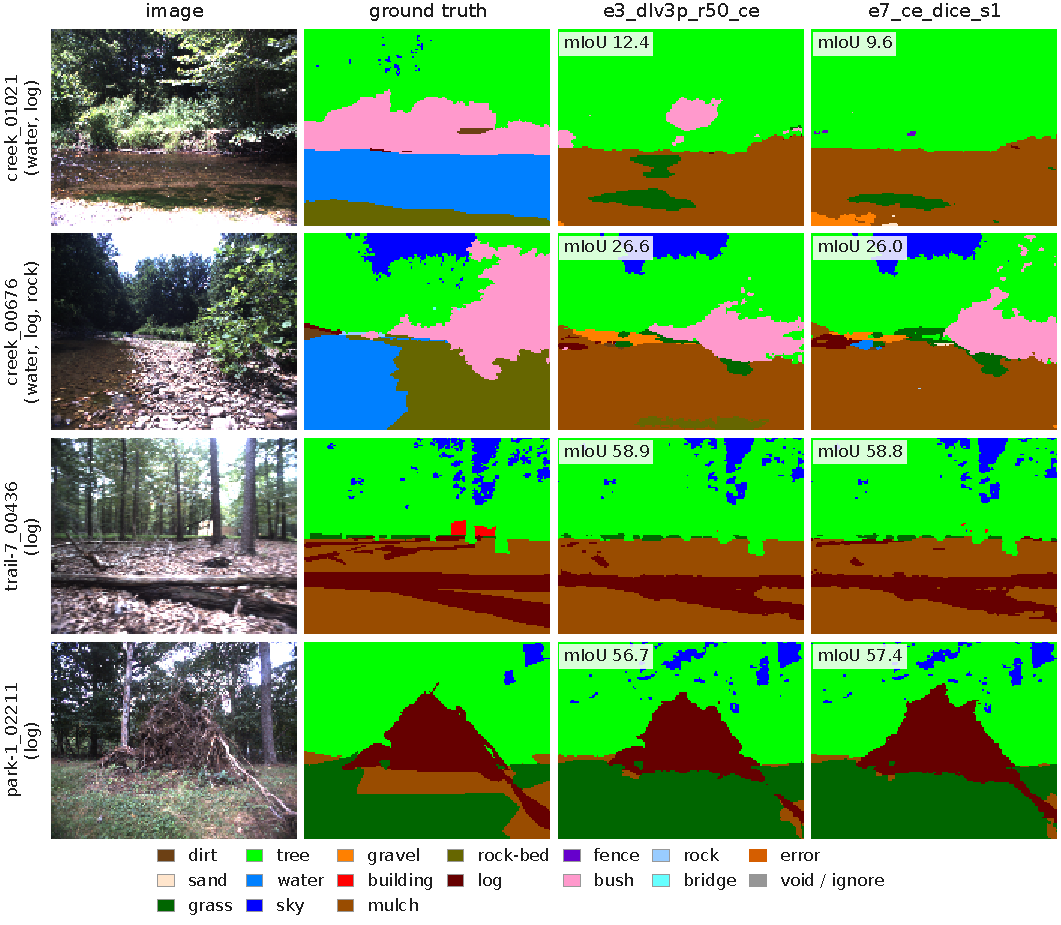
\includegraphics[width=0.82\textwidth]{../results/figures/compare_e3_dlv3p_r50_ce_vs_e7_ce_dice_s1_test.pdf}
  \caption{CE (E3) vs.\ CE+Dice (E7, seed 1) on test frames containing water,
  log, or rock, with per-frame mIoU. Rows 1--2 (creek): both models label the
  clear, shallow stream as mulch and the cobble bed (\emph{rock-bed}, olive) as
  mulch or gravel. Rows 3--4: logs are segmented well by both. In the official
  palette, \emph{concrete} and \emph{rock-bed} have nearly identical colors;
  no concrete appears in these frames.}
  \label{fig:gallery}
\end{figure*}

\begin{figure}[t]
  \centering
  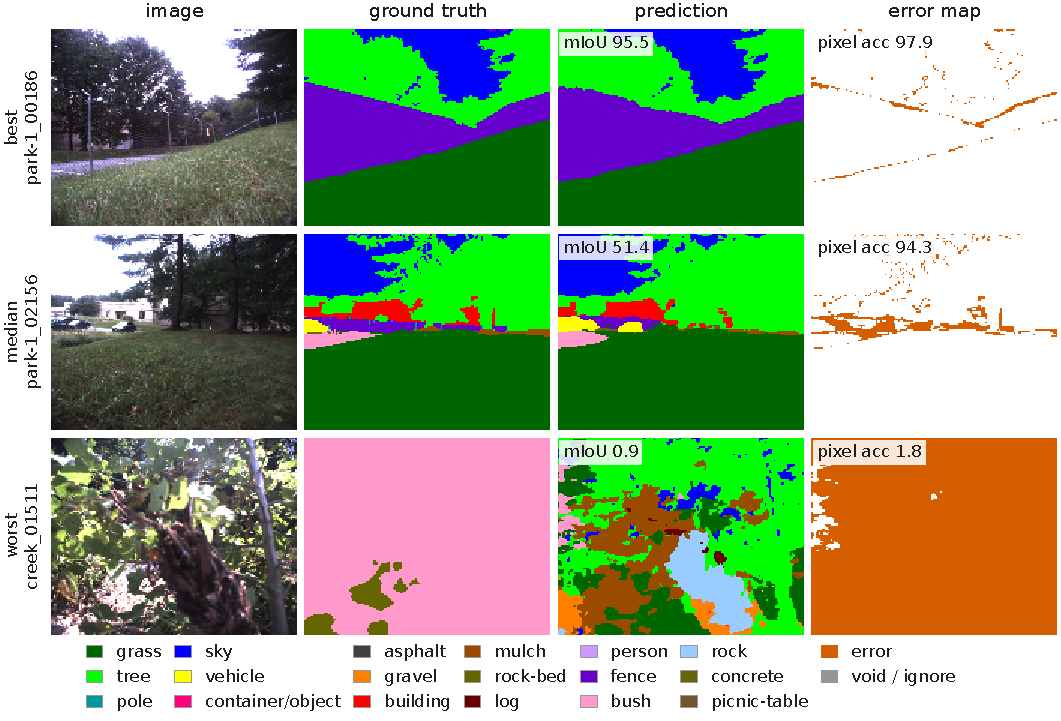
\includegraphics[width=\linewidth]{../results/figures/gallery_e7_ce_dice_s1_test.pdf}
  \caption{Best, median, and worst test frames of the final model by per-frame
  mIoU. Errors in good frames sit on class boundaries (fence edges, tree/sky
  transitions); the worst frame is a leaf close-up labeled \emph{bush}.}
  \label{fig:best_worst}
\end{figure}

\subsection{Boundary Ambiguity}

Excluding a 3-pixel band around label boundaries (at $384^2$), which holds
15\% of test pixels, raises the final model's test mIoU from 37.7\% to 40.8\%;
pixel accuracy is 79\% in the interior and 61\% in the band. Yet the band
holds only 26\% of test errors (13\% at 1\,px, 34\% at 5\,px). On validation,
by contrast, the same band holds 53\% of errors. Where the model recognizes the
scene, as in validation, most residual error lies at ambiguous transitions
(grass/mulch, bush/tree), consistent with the coarse polygon labels. On
test, most error comes from whole regions misrecognized in creek, which no
boundary tolerance can recover. The pattern is the same for every model
(Table~\ref{tab:main} models: 24--27\% of test errors in the 3\,px band).

\subsection{Classes the Data Cannot Support}

\emph{Bridge} illustrates a failure that no loss function can fix: with zero
training pixels, its roughly 4.6\,M native-resolution test pixels must be
assigned to some other class. The final model predicts \emph{vehicle} for 50\%
of them (CE: 71\%), then tree (19\%) and grass (8\%), the nearest learned
large man-made structure and its surroundings. Its IoU is 0 by construction.
\emph{Bicycle} is absent from test, and the final model predicts it on no test
pixel, so it does not enter the test mIoU.
